\chapter{Data-driven Landscapes of Colon Epithelial Plasticity}
\label{05vr}

\section{Introduction}

% In 1957, C.H. Waddington published his famous illustration of cellular differentiation, depicting pluripotent cells rolling down a landscape into valleys of terminal differentiation \cite{waddington_strategy_1957}. While an evocative metaphor in developmental biology, this conceptual model has not been clearly demonstrated with real data. However, recent computational advances in global-structure embeddings \cite{moon_visualizing_2019}, differentiation potency metrics \cite{teschendorff_singlecell_2017}, and local differentiation-rate predictions \cite{bergen_generalizing_2020} now provide the component elements to reconstruct Waddington-like embeddings from scRNA-seq data. 


\section{Valley-Ridge scores as a landscape of colonic epithelial cell-fate plasticity}

% To visualise single-cell colonic epithelial differentiation on a Waddington-like landscape, we combined the global cellular relationships captured by PHATE \cite{moon_visualizing_2019} as 'longitude and latitude' axes, with an integrated Valley-Ridge (VR) score to represent pluripotent 'altitude'. The VR score is defined as the sum of two components per cluster: CCAT signalling-entropy \cite{teschendorff_singlecell_2017} and RNA velocity \cite{bergen_generalizing_2020}. At a cluster's centre, the VR score is solely determined by the median CCAT. However, the VR scores at the cluster periphery were augmented by weighting the inverse of RNA velocity component and the scaled distance from the cluster centre to model rates of local transcriptional change. This method reconstructs a data-driven estimate of Waddington-like landscapes where the altitude captures the differentiation potential of a cell population, with the valley-ridge topology delineating local plasticity (Figure \ref{fig:fig6}A). 


\subsubsection{Figure on VR score definition}

\begin{figure}
    \centering
    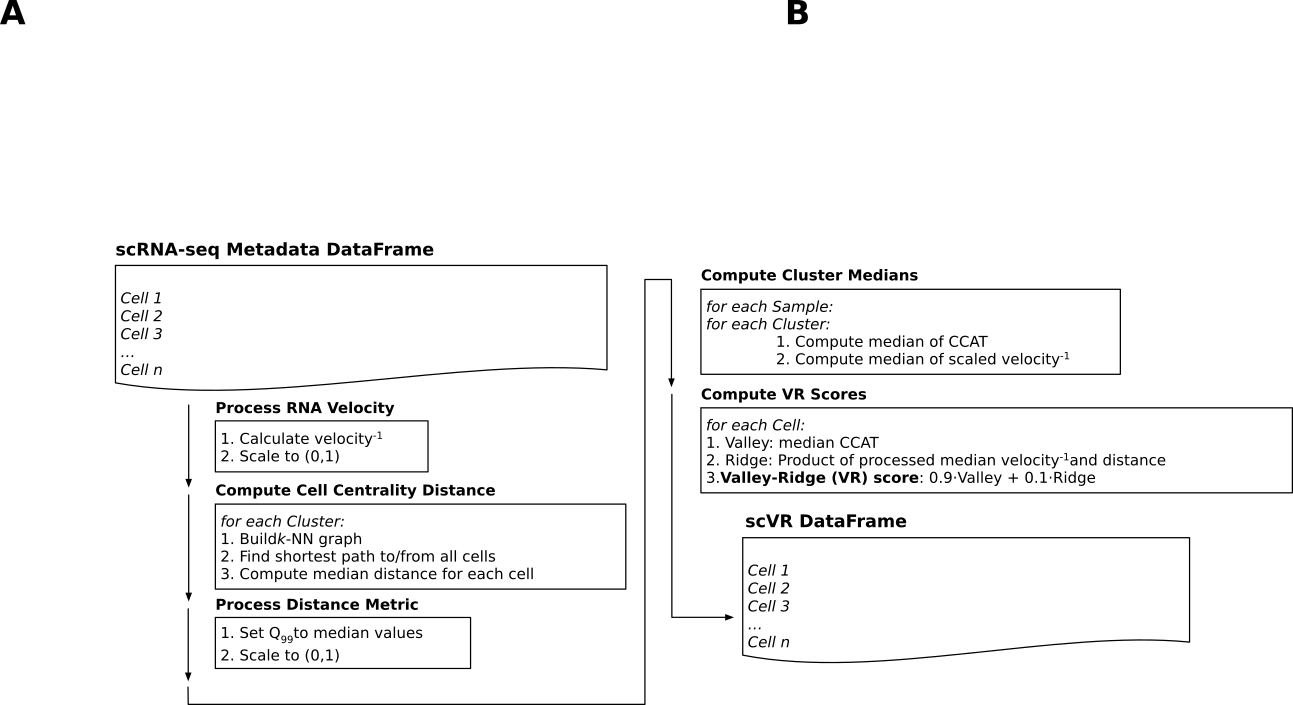
\includegraphics{05vr/figs/5VR_Score.png}
    \caption{}
    \label{fig:}
\end{figure}

Correlation of VR score with CCAT and with Origins for each cell, grouped by clusters

\section{Landascapes themselves}

% When WT colonic epithelia are projected onto this embedding, stem cells occupy high positions in the landscape, with TA cells descending into a central valley before diverging into terminally differentiated secretory and absorptive cells. When WT epithelia communicate with fibroblasts, the TA valley erodes as cells access revCSC. In contrast, CRC mutations \textit{shApc} and \textit{Kras\textsuperscript{G12D/+}} re-sculpt the entire landscape, trapping most cells in the proCSC fate by restricting their differentiation potential (Figure \ref{fig:fig6}A). 

\subsubsection{Figure on VR Waddington-like landscapes}

\begin{figure}
    \centering
    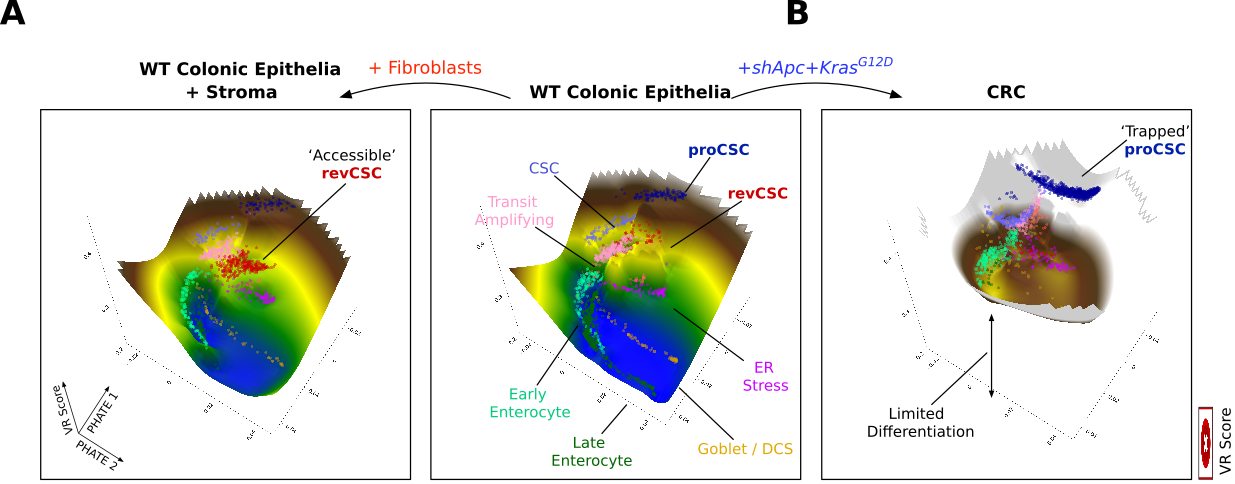
\includegraphics{05vr/figs/5VR_Landscape.png}
    \caption{}
    \label{fig:}
\end{figure}

\section{Conclusions}


% These observations demonstrate that colonic epithelia exist on an integrated differentiation landscape that can be traversed by co-regulating core signalling hubs, either through cell-intrinsic mutations or cell-extrinsic ligands. 


